\documentclass[tikz,border=10pt]{standalone}
% TikZ units: cm, origin at O, s = 0.013378 cm/px, y flipped
\usepackage{tikz}
\begin{document}
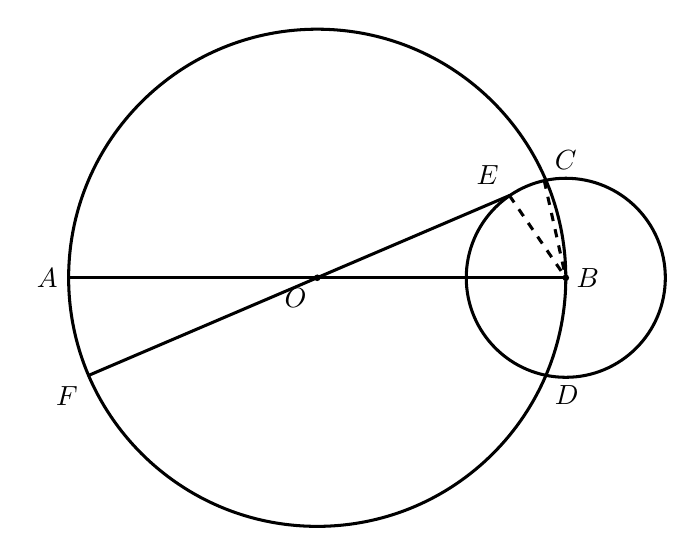
\begin{tikzpicture}[line width=1.1pt, line join=round]
  % Named coordinates (converted from pixels)
  \coordinate (O) at (0,0);
  \coordinate (A) at (-3.160,0);
  \coordinate (B) at (3.157,0);
  \coordinate (C) at (2.883,1.235);
  \coordinate (D) at (2.883,-1.237);
  \coordinate (E) at (2.441,1.044);
  \coordinate (F) at (-2.906,-1.241);

  % Circles: big centred at O (radius 3.157), small centred at B (radius 1.264)
  \draw (O) circle[radius=3.157];
  \draw (B) circle[radius=1.264];

  % Horizontal diameter A-B (solid)
  \draw (A) -- (B);

  % Solid line F through O to E
  \draw (F) -- (E);

  % Dashed segments E-B and C-B
  \draw[dashed] (E) -- (B);
  \draw[dashed] (C) -- (B);

  % Vertex dots and labels
  \fill (O) circle (1.2pt);
  \fill (B) circle (1.2pt);
  \node[left]        at (A) {\fontsize{10}{12}\selectfont $A$};
  \node[below left]  at (O) {\fontsize{10}{12}\selectfont $O$};
  \node[right]       at (B) {\fontsize{10}{12}\selectfont $B$};
  \node[above right] at (C) {\fontsize{10}{12}\selectfont $C$};
  \node[below right] at (D) {\fontsize{10}{12}\selectfont $D$};
  \node[above left]  at (E) {\fontsize{10}{12}\selectfont $E$};
  \node[below left]  at (F) {\fontsize{10}{12}\selectfont $F$};
\end{tikzpicture}
\end{document}